\documentclass{article}
\usepackage{tikz}
\usepackage{pgfplots}
\usepackage{textcomp}
\usepackage{array}
\usepackage{tabu}
\usepackage{numprint}
\begin{document}

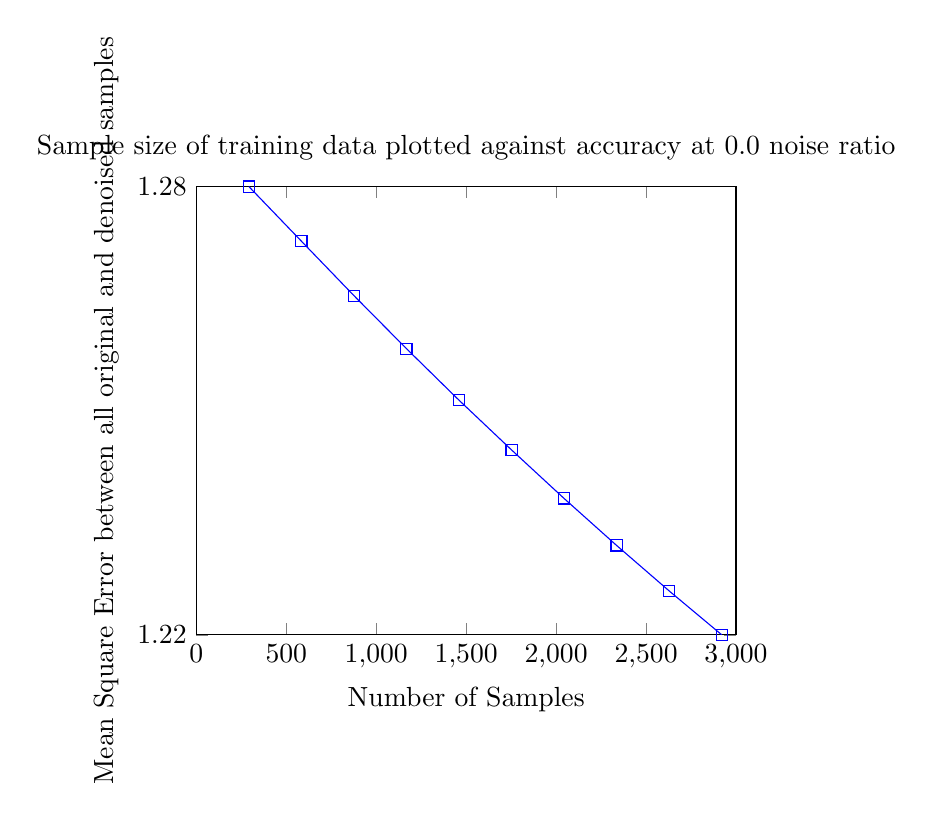
\begin{tikzpicture}
\begin{axis}[
title={Sample size of training data plotted against accuracy at 0.0 noise ratio},
xlabel={Number of Samples},
ylabel={Mean Square Error between all original and denoised samples},
xmin=0, xmax=3000,
ymin=1.2230914440164478, ymax=1.2800505560710056,
xtick={0,500,1000,1500,2000,2500,3000},
ytick={1.2230914440164478,1.2800505560710056},
legend pos=north west,
ymajorgrids=true,
grid style=dashed,
]

\addplot[
color=blue,
mark=square,
]
coordinates {

(292, 1.2800505560710056)
(584, 1.2731099324588)
(876, 1.2661913766561106)
(1168, 1.2594562378017642)
(1460, 1.2529105068279087)
(1752, 1.2465937007452959)
(2044, 1.240429258256478)
(2336, 1.2344579602946324)
(2628, 1.2286842941439895)
(2921, 1.2230914440164478)
    };
\end{axis}
\end{tikzpicture}

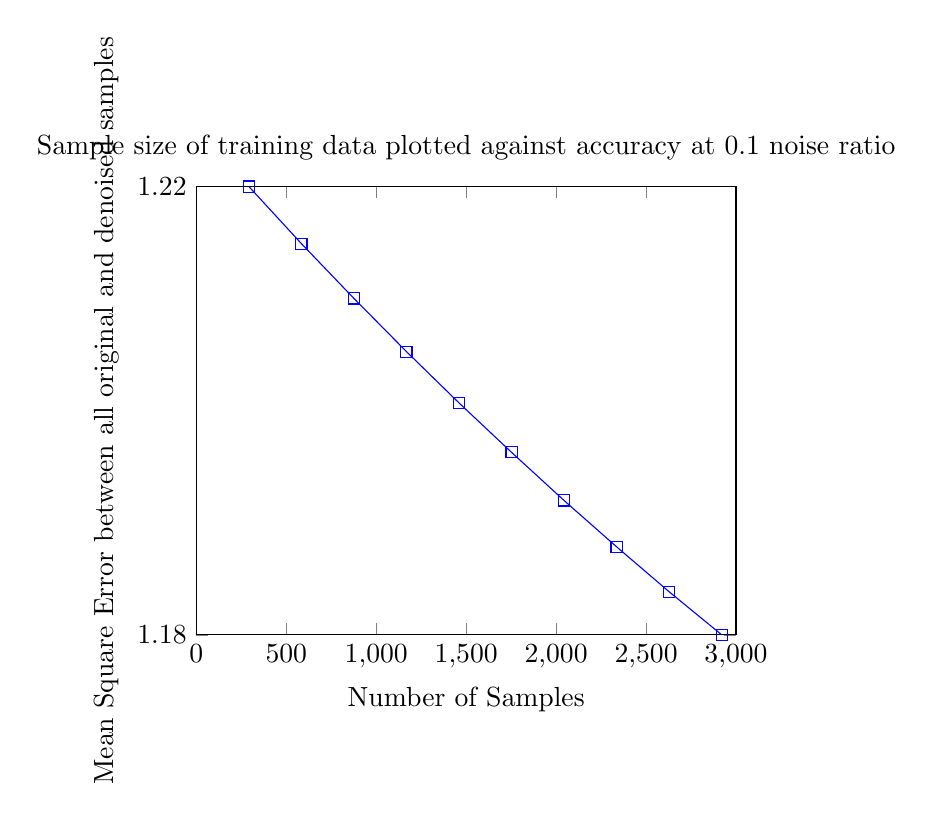
\begin{tikzpicture}
\begin{axis}[
title={Sample size of training data plotted against accuracy at 0.1 noise ratio},
xlabel={Number of Samples},
ylabel={Mean Square Error between all original and denoised samples},
xmin=0, xmax=3000,
ymin=1.1765378872141743, ymax=1.2176631613242135,
xtick={0,500,1000,1500,2000,2500,3000},
ytick={1.1765378872141743,1.2176631613242135},
legend pos=north west,
ymajorgrids=true,
grid style=dashed,
]

\addplot[
color=blue,
mark=square,
]
coordinates {

(292, 1.2176631613242135)
(584, 1.2124260070112693)
(876, 1.207399859979822)
(1168, 1.202523629941026)
(1460, 1.197817076328806)
(1752, 1.1932835915875017)
(2044, 1.1888672810350938)
(2336, 1.1846184641513644)
(2628, 1.1804982033474893)
(2921, 1.1765378872141743)
    };
\end{axis}
\end{tikzpicture}

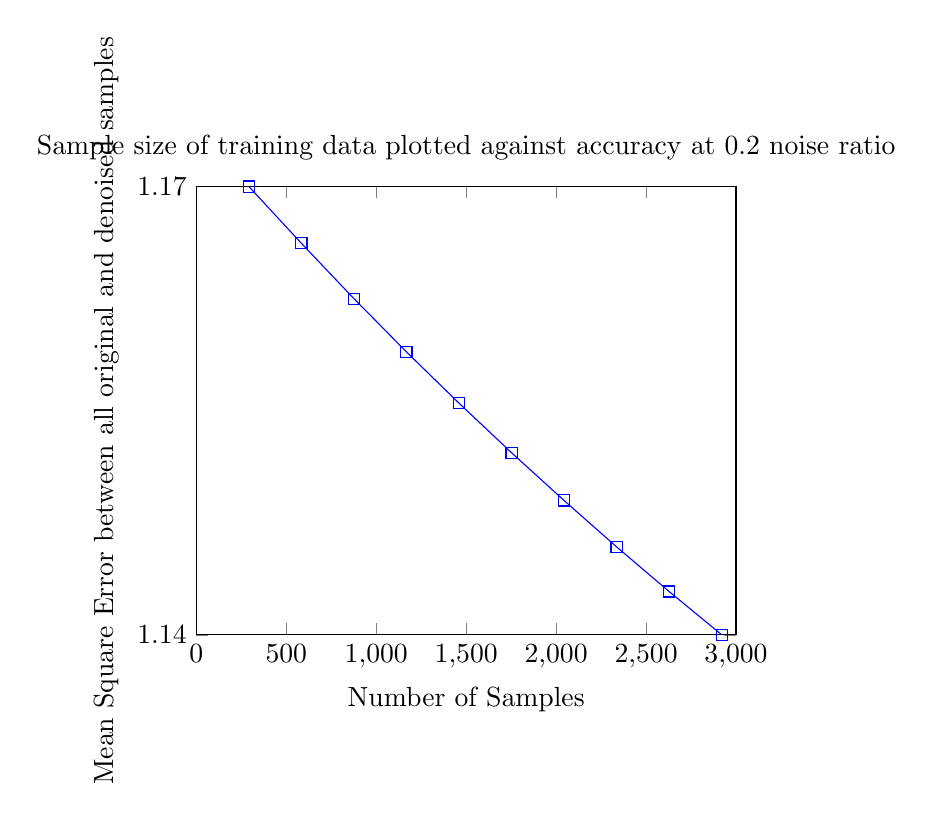
\begin{tikzpicture}
\begin{axis}[
title={Sample size of training data plotted against accuracy at 0.2 noise ratio},
xlabel={Number of Samples},
ylabel={Mean Square Error between all original and denoised samples},
xmin=0, xmax=3000,
ymin=1.1435365274851699, ymax=1.1726964753604965,
xtick={0,500,1000,1500,2000,2500,3000},
ytick={1.1435365274851699,1.1726964753604965},
legend pos=north west,
ymajorgrids=true,
grid style=dashed,
]

\addplot[
color=blue,
mark=square,
]
coordinates {

(292, 1.1726964753604965)
(584, 1.1690020846521134)
(876, 1.1654062728345032)
(1168, 1.1619402902421363)
(1460, 1.1586061639178835)
(1752, 1.1553851760059357)
(2044, 1.152279134032352)
(2336, 1.1492623134480224)
(2628, 1.1463584000040108)
(2921, 1.1435365274851699)
    };
\end{axis}
\end{tikzpicture}


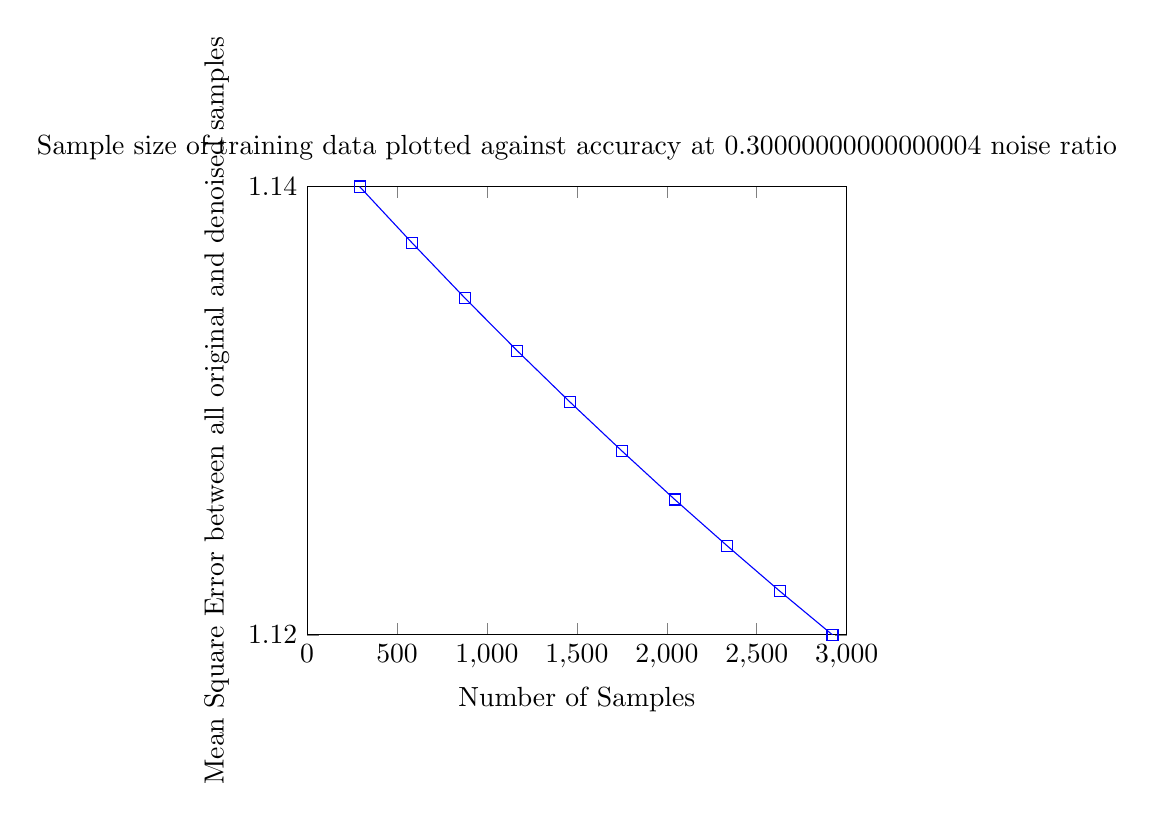
\begin{tikzpicture}
\begin{axis}[
title={Sample size of training data plotted against accuracy at 0.30000000000000004 noise ratio},
xlabel={Number of Samples},
ylabel={Mean Square Error between all original and denoised samples},
xmin=0, xmax=3000,
ymin=1.1199695987341185, ymax=1.1408188216709414,
xtick={0,500,1000,1500,2000,2500,3000},
ytick={1.1199695987341185,1.1408188216709414,1.1616680446077643},
legend pos=north west,
ymajorgrids=true,
grid style=dashed,
]

\addplot[
color=blue,
mark=square,
]
coordinates {

(292, 1.1408188216709414)
(584, 1.1381973937129914)
(876, 1.135647752263494)
(1168, 1.1331854256062863)
(1460, 1.1308112731242197)
(1752, 1.1285091280243424)
(2044, 1.1262662323148451)
(2336, 1.1241064713808309)
(2628, 1.1220040148363126)
(2921, 1.1199695987341185)
    };
\end{axis}
\end{tikzpicture}

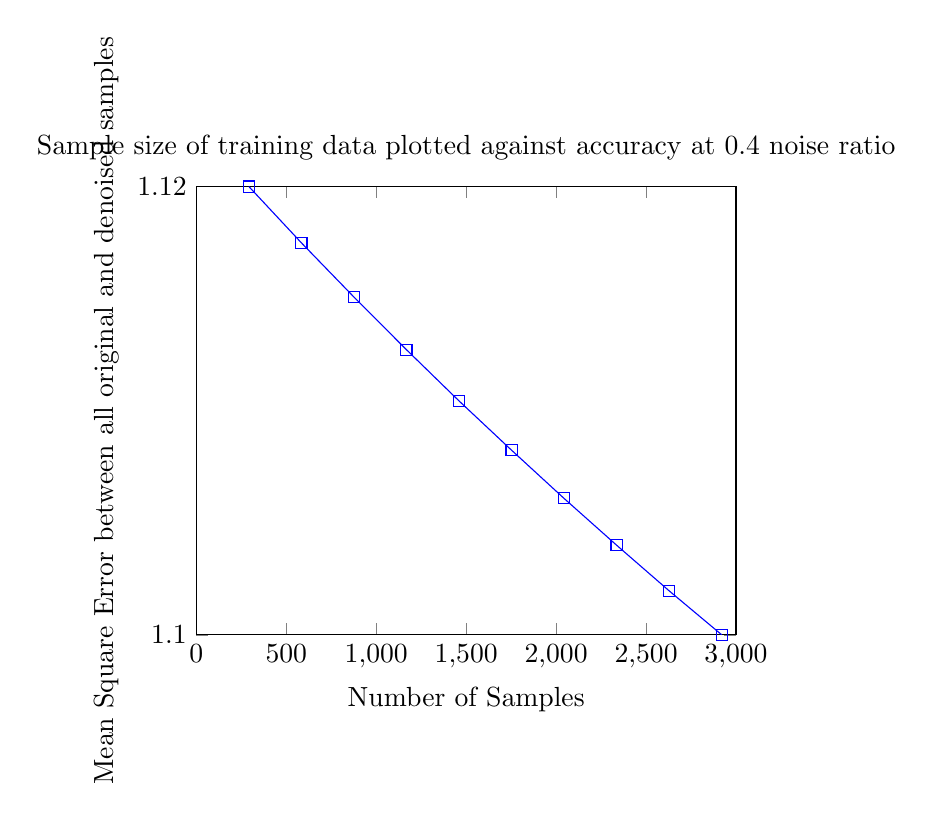
\begin{tikzpicture}
\begin{axis}[
title={Sample size of training data plotted against accuracy at 0.4 noise ratio},
xlabel={Number of Samples},
ylabel={Mean Square Error between all original and denoised samples},
xmin=0, xmax=3000,
ymin=1.102731253965157, ymax=1.1179959752183977,
xtick={0,500,1000,1500,2000,2500,3000},
ytick={1.102731253965157,1.1179959752183977},
legend pos=north west,
ymajorgrids=true,
grid style=dashed,
]

\addplot[
color=blue,
mark=square,
]
coordinates {

(292, 1.1179959752183977)
(584, 1.1160786728637906)
(876, 1.1142342231041802)
(1168, 1.1124405022141752)
(1460, 1.1106982443664017)
(1752, 1.1090208828829244)
(2044, 1.1073780657924521)
(2336, 1.105785879818721)
(2628, 1.1042325383690896)
(2921, 1.102731253965157)
    };
\end{axis}
\end{tikzpicture}

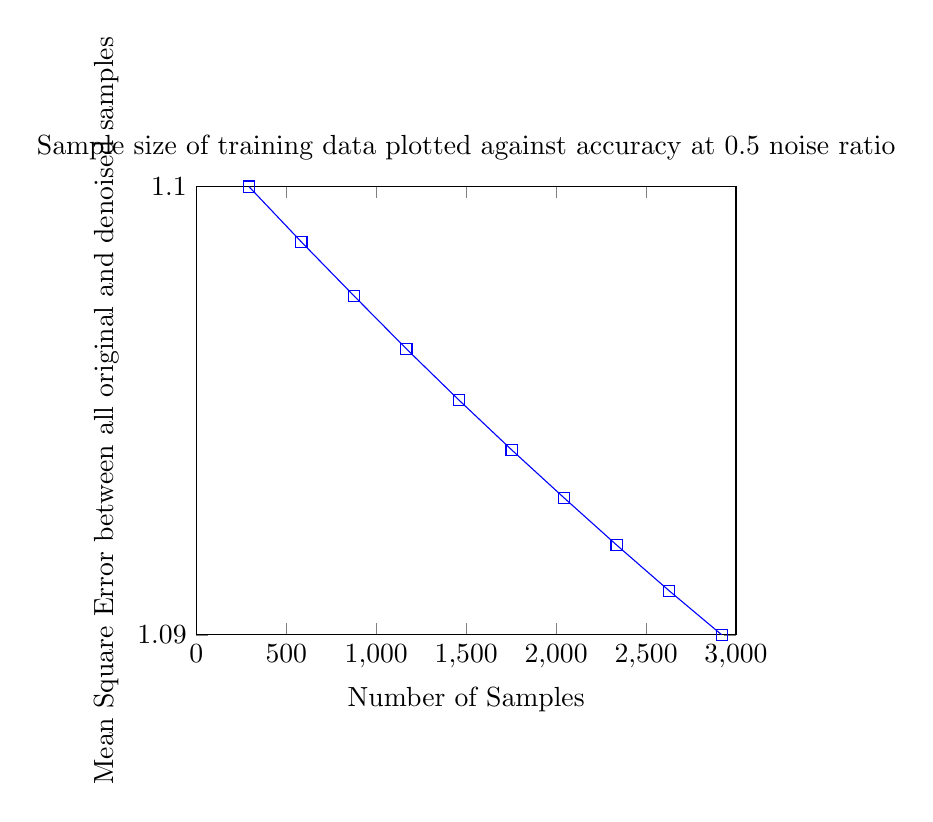
\begin{tikzpicture}
\begin{axis}[
title={Sample size of training data plotted against accuracy at 0.5 noise ratio},
xlabel={Number of Samples},
ylabel={Mean Square Error between all original and denoised samples},
xmin=0, xmax=3000,
ymin=1.0898148822081117, ymax=1.1012885571290247,
xtick={0,500,1000,1500,2000,2500,3000},
ytick={1.0898148822081117,1.1012885571290247},
legend pos=north west,
ymajorgrids=true,
grid style=dashed,
]

\addplot[
color=blue,
mark=square,
]
coordinates {

(292, 1.1012885571290247)
(584, 1.099870591672322)
(876, 1.0984922016121383)
(1168, 1.097132893822148)
(1460, 1.0958228836512396)
(1752, 1.0945538486799409)
(2044, 1.0933219659815496)
(2336, 1.092115585991027)
(2628, 1.0909453046786988)
(2921, 1.0898148822081117)
    };
\end{axis}
\end{tikzpicture}

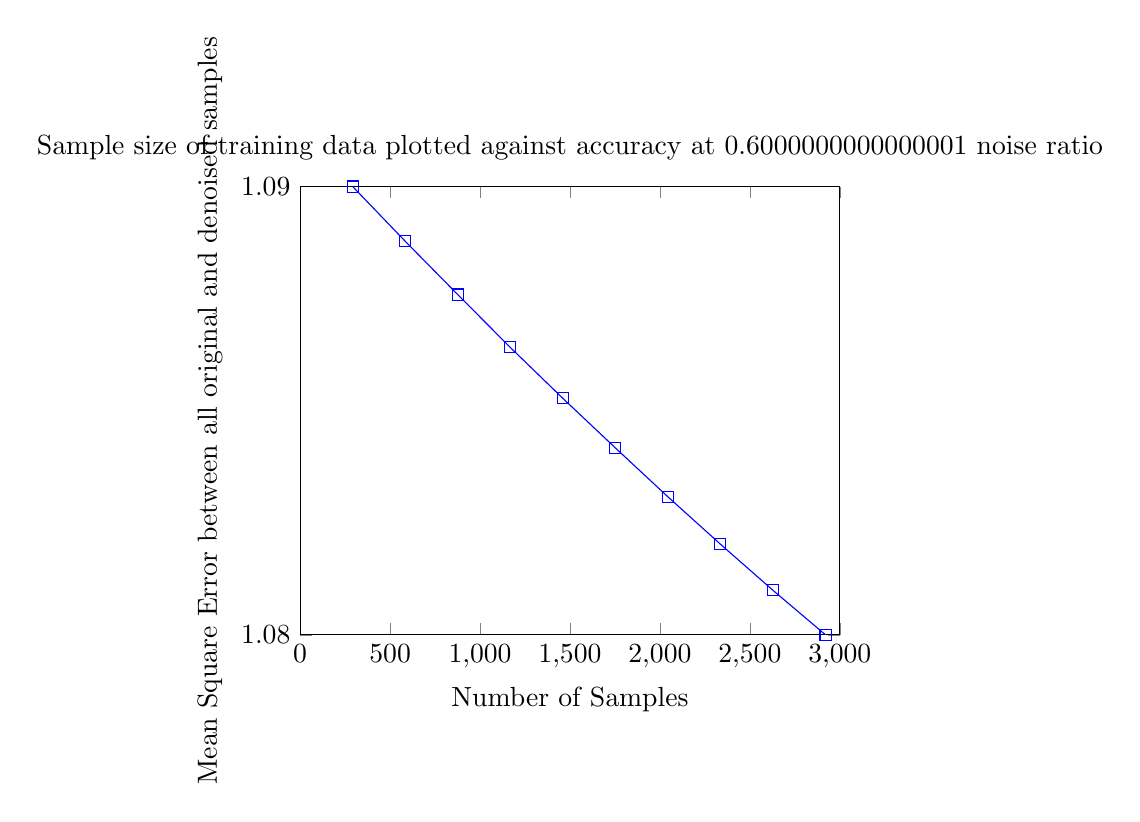
\begin{tikzpicture}
\begin{axis}[
title={Sample size of training data plotted against accuracy at 0.6000000000000001 noise ratio},
xlabel={Number of Samples},
ylabel={Mean Square Error between all original and denoised samples},
xmin=0, xmax=3000,
ymin=1.0799317121327823, ymax=1.0887156592833784,
xtick={0,500,1000,1500,2000,2500,3000},
ytick={1.0799317121327823,1.0887156592833784},
legend pos=north west,
ymajorgrids=true,
grid style=dashed,
]

\addplot[
color=blue,
mark=square,
]
coordinates {

(292, 1.0887156592833784)
(584, 1.08764427747387)
(876, 1.086599070577405)
(1168, 1.0855649867552142)
(1460, 1.0845675426469423)
(1752, 1.083596402106567)
(2044, 1.0826381787394128)
(2336, 1.0817100765080172)
(2628, 1.0808064513642652)
(2921, 1.0799317121327823)
    };
\end{axis}
\end{tikzpicture}

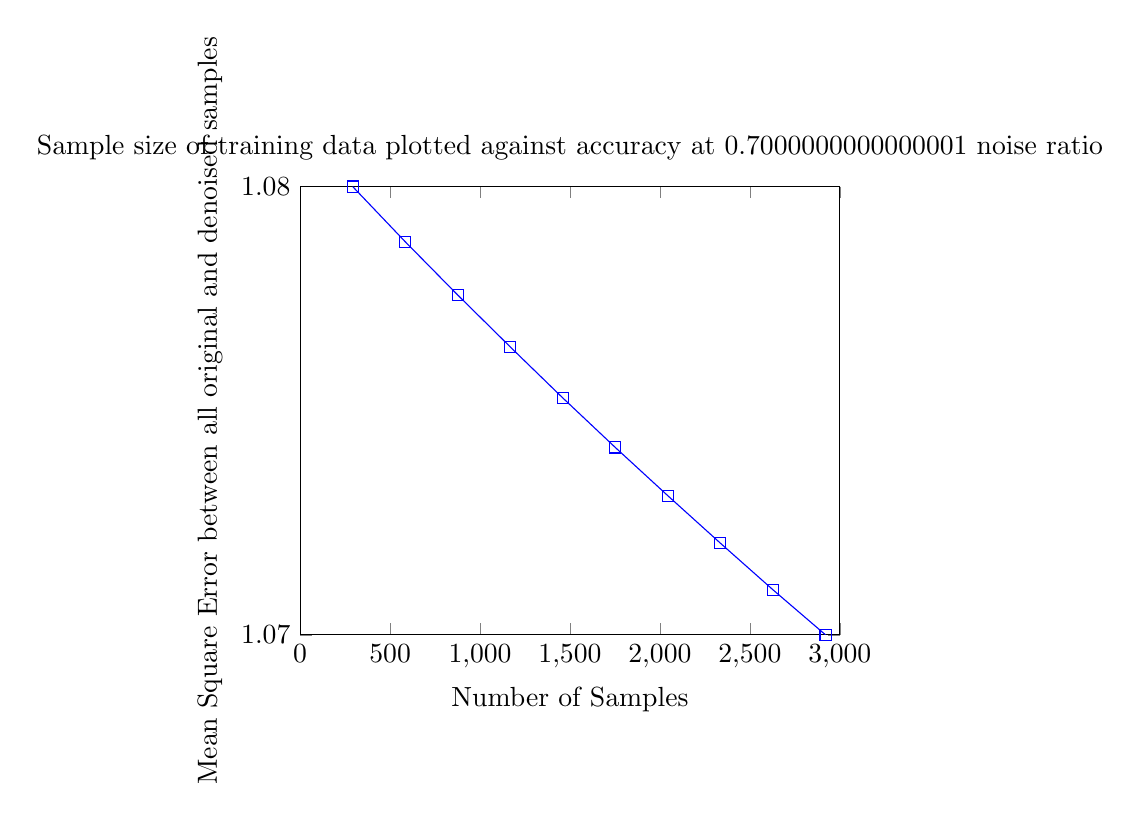
\begin{tikzpicture}
\begin{axis}[
title={Sample size of training data plotted against accuracy at 0.7000000000000001 noise ratio},
xlabel={Number of Samples},
ylabel={Mean Square Error between all original and denoised samples},
xmin=0, xmax=3000,
ymin=1.0721515911206394, ymax=1.0790553230245687,
xtick={0,500,1000,1500,2000,2500,3000},
ytick={1.0721515911206394,1.0790553230245687},
legend pos=north west,
ymajorgrids=true,
grid style=dashed,
]

\addplot[
color=blue,
mark=square,
]
coordinates {

(292, 1.0790553230245687)
(584, 1.078206052287615)
(876, 1.0773853553457422)
(1168, 1.0765861149415927)
(1460, 1.0758005478709223)
(1752, 1.0750379234726595)
(2044, 1.0742946892427359)
(2336, 1.073564333811611)
(2628, 1.0728472057779626)
(2921, 1.0721515911206394)
    };
\end{axis}
\end{tikzpicture}

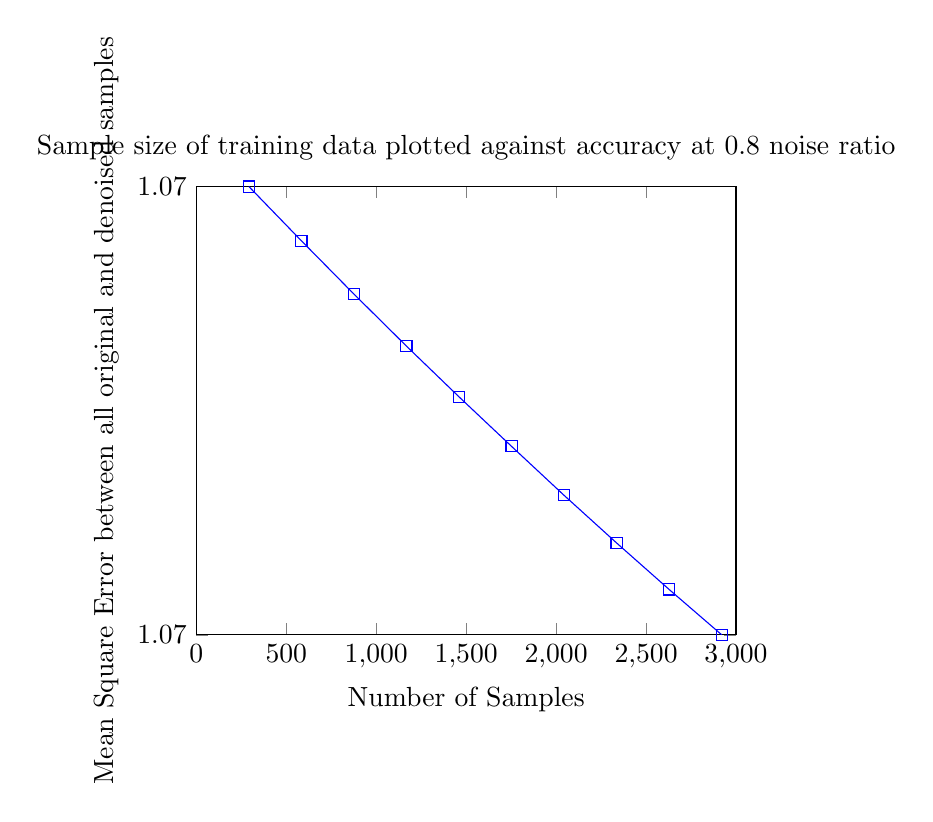
\begin{tikzpicture}
\begin{axis}[
title={Sample size of training data plotted against accuracy at 0.8 noise ratio},
xlabel={Number of Samples},
ylabel={Mean Square Error between all original and denoised samples},
xmin=0, xmax=3000,
ymin=1.0659469455013324, ymax=1.0714782917720165,
xtick={0,500,1000,1500,2000,2500,3000},
ytick={1.0659469455013324,1.0714782917720165},
legend pos=north west,
ymajorgrids=true,
grid style=dashed,
]

\addplot[
color=blue,
mark=square,
]
coordinates {

(292, 1.0714782917720165)
(584, 1.070808872716178)
(876, 1.070151477501708)
(1168, 1.0695095508728625)
(1460, 1.0688840911358117)
(1752, 1.068273235375066)
(2044, 1.0676690646979006)
(2336, 1.0670814634459727)
(2628, 1.0665078535019716)
(2921, 1.0659469455013324)
    };
\end{axis}
\end{tikzpicture}

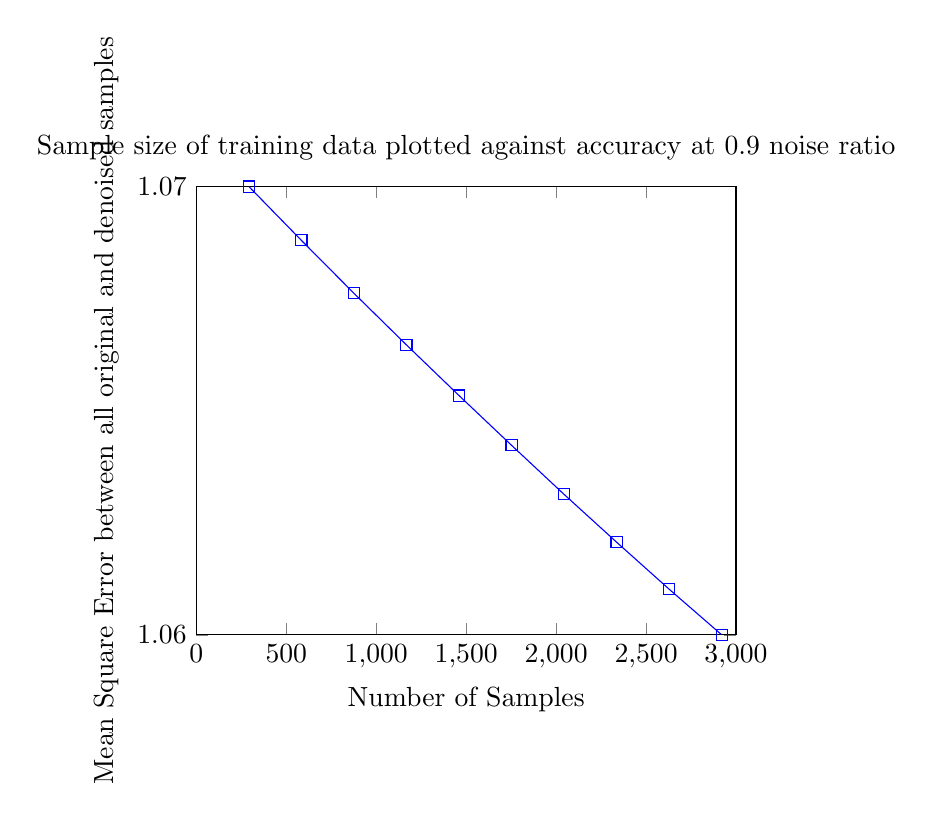
\begin{tikzpicture}
\begin{axis}[
title={Sample size of training data plotted against accuracy at 0.9 noise ratio},
xlabel={Number of Samples},
ylabel={Mean Square Error between all original and denoised samples},
xmin=0, xmax=3000,
ymin=1.0608927701657307, ymax=1.0653819348346338,
xtick={0,500,1000,1500,2000,2500,3000},
ytick={1.0608927701657307,1.0653819348346338},
legend pos=north west,
ymajorgrids=true,
grid style=dashed,
]

\addplot[
color=blue,
mark=square,
]
coordinates {

(292, 1.0653819348346338)
(584, 1.0648428422246163)
(876, 1.0643131958733343)
(1168, 1.0637960196719944)
(1460, 1.0632895641386546)
(1752, 1.0627914127806257)
(2044, 1.0623000263291724)
(2336, 1.0618213036492006)
(2628, 1.0613506540666822)
(2921, 1.0608927701657307)
    };
\end{axis}
\end{tikzpicture}

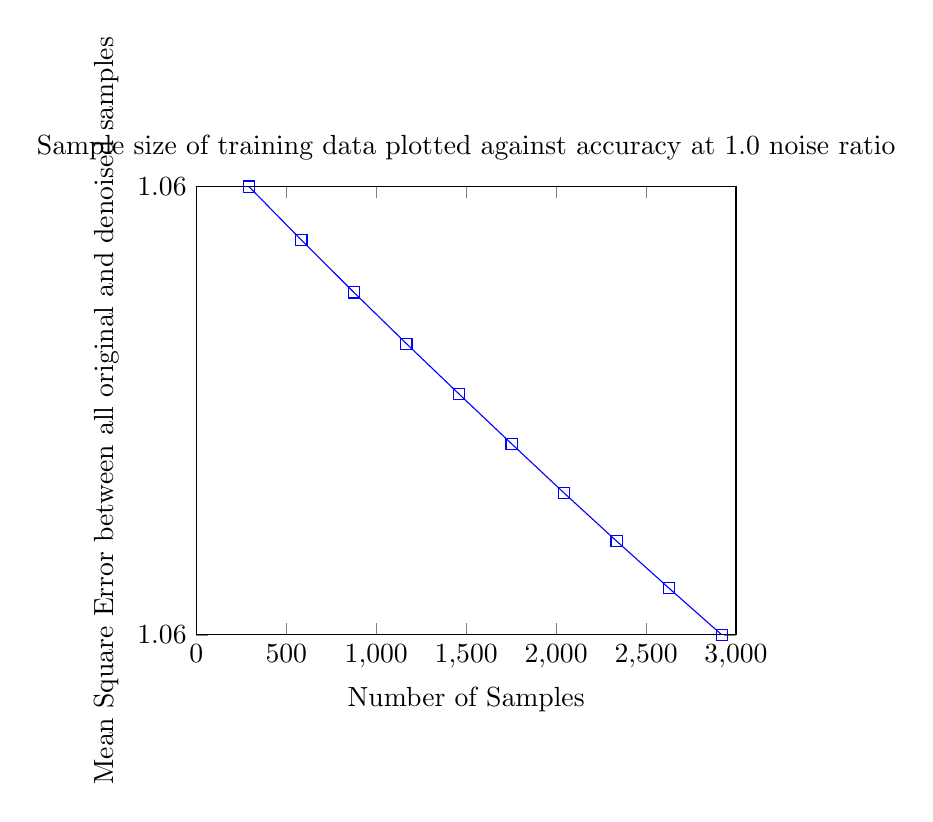
\begin{tikzpicture}
\begin{axis}[
title={Sample size of training data plotted against accuracy at 1.0 noise ratio},
xlabel={Number of Samples},
ylabel={Mean Square Error between all original and denoised samples},
xmin=0, xmax=3000,
ymin=1.056729968184138, ymax=1.0604429416422594,
xtick={0,500,1000,1500,2000,2500,3000},
ytick={1.056729968184138,1.0604429416422594},
legend pos=north west,
ymajorgrids=true,
grid style=dashed,
]

\addplot[
color=blue,
mark=square,
]
coordinates {

(292, 1.0604429416422594)
(584, 1.0600000550695041)
(876, 1.059566185313775)
(1168, 1.0591413955218116)
(1460, 1.0587252505249538)
(1752, 1.0583132383710232)
(2044, 1.0579051849648908)
(2336, 1.0575068441832303)
(2628, 1.0571162215046872)
(2921, 1.056729968184138)
    };
\end{axis}
\end{tikzpicture}
\end{document}